% Author: Dr. Matthias Jung, DL9MJ
% Year: 2021
\documentclass[convert = false, border=5pt]{standalone}
\usepackage{fontspec}
\setmainfont{Roboto}
\usepackage[siunitx, straightvoltages, europeanresistors, european inductor]{circuitikzgit}
\usepackage{tikz}


\usetikzlibrary{calc, positioning}

\begin{document}
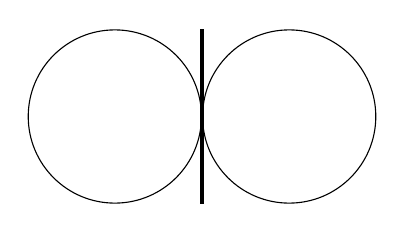
\begin{tikzpicture}[
   node distance = 0pt,
     circ/.style = {circle, draw, minimum size=22mm,
                    node contents={}},
every pin/.style = {align=center}
                    ]
  \node (n1) [circ];
  \node (n2) [circ,right=of n1];
    \draw [very thick]
        (n1.north -| n1.east) -- (n1.south -| n1.east)
        node[below] {};
\end{tikzpicture}
\end{document}
